\documentclass[11pt, a4paper]{article}

% Languages and fonts
\usepackage{cmap} 
\usepackage[T2A]{fontenc}
\usepackage[utf8]{inputenc} 
\usepackage[english, russian]{babel}
\usepackage{microtype}
\usepackage{indentfirst}
\frenchspacing

% Mathematics
\usepackage{amsmath, amssymb, amsfonts, amsthm, mathtools, fixmath}
\mathtoolsset{showonlyrefs=true}
\usepackage{esint, esvect} % integrals and vectors
\usepackage{systeme} % equation system
\usepackage{commath} % partials and differentials
\usepackage{icomma} % smart comma ($0,2$ is a number)

% Floats
\usepackage{float}

% Tables
\usepackage{array,tabularx,tabulary,booktabs} % better tables
\usepackage{longtable}
\usepackage{multirow}

% Graphics
\usepackage[pdftex]{graphicx}
\usepackage{wrapfig}

% Theorems
\renewcommand{\proofname}{Доказательство}

\theoremstyle{plain}
\newtheorem{theorem}{Теорема}[section]

\theoremstyle{definition}
\newtheorem{definition}{Определение}
\newtheorem{corollary}{Следствие}[theorem]
\newtheorem{problem}{Задача}[section]

\theoremstyle{remark}
\newtheorem{remark}{Замечание}
\newtheorem*{solution}{Решение}

\usepackage[top=20mm,bottom=20mm,left=20mm,right=20mm]{geometry}

\usepackage{lastpage} % how many pages

\usepackage{soul}

\usepackage{framed} % easy frames
\usepackage{enumerate} % better numbered lists

\usepackage{hyperref}
\usepackage{xcolor}

\usepackage{tikz} % drawing

\usepackage{csquotes}
\usepackage[style=numeric,backend=biber,sorting=none]{biblatex}
\addbibresource{../../../../bibliography.bib}

\renewcommand{\epsilon}{\ensuremath{\varepsilon}}
\renewcommand{\phi}{\ensuremath{\varphi}}
\renewcommand{\theta}{\vartheta}
\renewcommand{\kappa}{\ensuremath{\varkappa}}
\renewcommand{\le}{\ensuremath{\leqslant}}
\renewcommand{\leq}{\ensuremath{\leqslant}}
\renewcommand{\ge}{\ensuremath{\geqslant}}
\renewcommand{\geq}{\ensuremath{\geqslant}}

\usepackage[useregional]{datetime2}

% custom maketitle
\usepackage{titling}
\setlength{\droptitle}{-4em}
\posttitle{\end{center}\vspace{-3em}}

\title{{\Large Геодезическая гравиметрия 2018}\\ 
    {\bf\Large Практическое занятие № 1} \\
{\Large Введение. Краткие сведения из математики и высшей геодезии}}
\author{}
\DTMsavedate{lessondate}{2018-02-13}
\date{\DTMusedate{lessondate}}

\begin{document}
\maketitle

\section{Организационные вопросы}

Курс <<Геодезическая гравиметрия>> читается на третьем (весенний семестр) и четвёртом
(осенний семестр) курсах для студентов геодезического факультета МИИГАиК направления «Геодезия и
дистанционное зондирование» (бакалавриат).

Весенний семестр посвящен изучению поля тяготения и его свойств, а также измерениям силы тяжести на
поверхности Земли. 
Осенний семестр будет включать в себя вопросы моделирования гравитационного поля Земли и решение
геодезических задач с использованием информации о гравитационном поле Земли.

\subsection{Контакты}

Канал в Телеграм (для оповещений и анонсов):
\href{https://t.me/miigaik_gravimetry_course_2018}{miigaik\_gravimetry\_course\_2018}

Почта: \href{mailto:oshchepkov@miigaik.ru}{oshchepkov@miigaik.ru}

Материалы курса доступны в git-репозитории на GitHub:
\href{https://github.com/ioshchepkov/physical-geodesy-courses}{ioshchepkov/physical-geodesy-courses}\\

Репозиторий находится в стадии наполнения и будет обновляться по ходу курса.

\subsection{Примерная программа практических занятий (весенний семестр)}
\begin{enumerate}
    \item Введение. Краткие сведения из математики и высшей геодезии.
    \item Притяжение. Основные понятия и свойства.
    \item Притяжение тел простой формы I.
    \item Притяжение тел простой формы II.
    \item Притяжение тел сложной формы. Гармонические функции.
    \item Гравитационное поле Земли и планет. Общая характеристика.
    \item Гравитационное поле Земли и планет. Изменение гравитационного поля во времени.
    \item Наземные методы и средства измерений. Абсолютные измерения силы тяжести.
    \item Статический метод измерения силы тяжести.
    \item Исследования статических гравиметров I.
    \item Исследования статических гравиметров II.
    \item Метрология. Сравнения и эталонирование гравиметров.
    \item Гравиметрический рейс.
    \item Обработка гравиметрического рейса. Гравиметрические сети.
\end{enumerate}

\subsection{Контроль знаний и выставление оценок}
В курсе (весенний семестр) предусмотрены следующие формы контроля знаний: 
\begin{itemize}
    \item лабораторные работы,
    \item домашние задания,
    \item самостоятельные работы,
    \item контрольные работы,
    \item зачёт.
\end{itemize}

На практических занятиях будут разбираться основные понятия для закрепления теоретического материала
лекций, а также будут решаться и разбираться простейшие и/или типовые примеры и задачи.
\textbf{Только} на
практических занятиях будут выполняться лабораторные работы с гравиметрами и разбираться отдельные
темы по разделу курса <<гравиметрия>>. Пропуски занятий с гравиметрами не допускаются, ибо в связи с
большим числом студентов и ограниченным числом преподавателей, у нас нет возможности заниматься с
вами вне аудиторных часов. Лабораторные работы с гравиметрами должны быть аккуратно оформлены и
защищены. Оцениваются работы по двоичной системе (зачёт/незачёт).

\subsubsection{Домашние задания}
Домашние задания (ДЗ) будут выдаваться после (почти) каждого практического занятия и будут
состоять из контрольных вопросов, обязательных типовых задач, а также дополнительных задач
повышенной сложности. Каждый вопрос и каждая задача в задании будут иметь свою «стоимость» в баллах.
Общая оценка за одно домашнее задание равна сумме баллов за все вопросы, примеры и задачи.
Максимальное число баллов за каждое домашнее задание --- $5,0$. Баллы, заработанные за решение задач
повышенной сложности могут быть зачтены в другие задания и формы контроля. Все домашние задания
должны быть защищены, что включает в себя несколько контрольных вопросов по теме и/или ходу решения.
Незащищённые задания не могут быть зачтены. Крайний срок сдачи --- две недели с момента выдачи
задания. После дедлайна домашние задания не принимаются и могут полностью войти в программу зачёта
для несдавшего студента. Задания можно высылать как в электронном (что крайне приветствуется) виде
вне занятий, так и сдавать их в рукописном виде в часы занятий. За использование системы
компьютерной вёрстки \LaTeX (читается как латех) при сдаче работ будет начисляться дополнительный балл.

\subsubsection{Самостоятельные работы}
Самостоятельные работы (СР) будут проводиться в течение 5 -- 8 минут в начале (почти) каждого
практического занятия по пройденному материалу, включая лекции. Они будут состоять из 2--3 вопросов
и/или простых задач. Максимальное число баллов за одну самостоятельную~---~$5,0$. 

\subsubsection{Контрольные работы}
В середине семестра будет проведена первая (КР№1) контрольная работа (КР), а в конце семестра
-- вторая (КР№2). Обе продолжительностью в один академический час (половина пары). Программа
контрольных будет включать в себя теоретические и практические вопросы по пройденному материалу, в
том числе лекционному. Максимальное число баллов за контрольную --- $5,0$.\par
Сдача обеих контрольных работ на положительную оценку ($\geq 3,0$) является условием допуска 
студента к зачёту.

\subsubsection{Зачёт}
При условии всех сданных и защищённых лабораторных работах, итоговая оценка за семестр выставляется
следующим образом. По всем видам контроля выводятся средние оценки, которые затем подставляются в
выражение

\begin{equation*}
    \text{О\_И = 0,5*О\_ДЗ + 0,2*О\_СР + 0,3*О\_КР},
\end{equation*}

где О\_И – итоговая оценка, О\_ДЗ – средняя оценка по домашним заданиям, О\_СР – средняя оценка по
самостоятельным работам, О\_КР – средняя оценка по двум контрольным.

Если итоговая оценка на конец семестра получается не менее 4,0 ($\text{О\_И} >= 4,0$), то студент получает
\textbf{зачёт автоматом}. 

К зачету студент собирает портфолио, то есть всё, что он сделал за семестр:
\begin{itemize}
    \item лабораторные работы;
    \item домашние задания;
    \item дополнительные задания, если имеются;
    \item конспекты практических занятий и лекций;
    \item контрольные работы, независимо от оценки.
\end{itemize}

Зачёт будет состоять из письменной и устной части. Письменно студент выполняет задания, по
которым за семестр он получил неудовлетворительную ($< 3,0$) оценку (прежде всего -- контрольные
работы). Устная часть включает вопросы по практическим и лекционным занятиям.

\subsubsection{Теоретический минимум}
Особое внимание необходимо обратить на вопросы теоретического минимума. Незнание уверенных
ответов на них автоматически влечёт за собой неудовлетворительную оценку ($0,0$) по всем видам
контроля знаний (домашние задания, самостоятельные и контрольные работы, зачёт). Обратное неверно,
знание ответов только на эти вопросы зачёта не гарантирует. Вопросы из этого списка будут
включаться в контроль по мере их появления в курсе.

\subsubsection{Бонусы}

При желании, студенту могут быть даны дополнительные <<творческие>> задания, которые могут быть
выполнены как индивидуально, так и коллективно (2--3 человека). За выполнение таких заданий будут
начисляться бонусные баллы. Штрафных санкций не предусмотрено.

\subsection{Литература}
\begin{refsection}
    \nocite{Shimbirev1975, Ogorodova2013, Yuzefovich2014}
    \printbibliography[title={\normalsize Рекомендуемая литература}]
\end{refsection}
\begin{refsection}
    \nocite{Yuzefovich1980, Torge1999, Ogorodova2006, Pellinen1978, Moritz2007, Moritz1983, Ogorodova2011}
    \printbibliography[title={\normalsize Дополнительная литература}]
\end{refsection}

\section{Предмет и задачи курса}
Вспомним, что основной научной задачей геодезии является определение фигуры и внешнего
гравитационного поля Земли и их изменений во времени. 

Геодезическая гравиметрия решает эту задачу
преимущественно на основе гравиметрических данных (то есть по измерениям величин,
характеризующих гравитационное поле Земли), изучая взаимосвязь фигуры Земли и её гравитационного
поля на поверхности. 
Геодезическую гравиметрию можно рассматривать как теоретический фундамент геодезии.
\footnote{Огородова, Л. В. Геодезическая гравиметрия // 
    Большая российская энциклопедия. Том~6. Москва, 2006, стр.~595}
Синонимами являются дисциплины <<физическая геодезия>> и <<теория фигуры Земли>>.
Решением той же задачи, но с использованием всей
совокупности существующих исходных данных (например, спутниковых) занимается теоретическая
геодезия, которая преподается обычно на последних курсах геодезических специальностей.

Другое определение можно сформулировать так: геодезическая гравиметрия ---
раздел геодезии, в котором рассматриваются теории и методы использования гравиметрических данных 
для решения научных и практических задач геодезии.
\footnote{Юркина, М. И. Геодезическая гравиметрия // Большая советская энциклопедия. --- М.:
Советская энциклопедия. 1969--1978. (в оригинале вместо <<гравиметрических данных>> ---
<<результатов измерения силы тяжести>>)}

Задача получения гравиметрических данных с необходимой плотностью и точностью стоит 
перед другой наукой, которая называется <<гравиметрия>> (или <<экспериментальная гравиметрия>>).

Вообще говоря, задача изучения внешнего гравитационного поля Земли в сущности является задачей
гефизики также, как и изучение магнитного поля (теория которого очень близка к гравитационному) 
и других физических полей. Но, как мы увидим по ходу курса, внешнее гравитационное поле и фигура
Земли на самом деле определяются одновременно из обработки одних и тех же исходных данных. Более
того, эти задачи неотделимы друг от друга, а потому и входят в основную задачу геодезии и её подразделов\cite{Pellinen1978}.

Действительно, ведь абсолютно все (<<геометрические>>) геодезические измерения выполняются в гравитационном поле 
Земли и связаны с ним. В этом легко убедиться, ответив на вопросы:
\begin{enumerate}
    \item Назовите основные геометрические условия в нивелирах и угломерных приборах.
    \item Что происходит с геодезическими приборами, когда мы выставляем их по уровням? 
    \item В какой системе координат выполняются измерения на поверхности Земли?
    \item Чему равна сумма измеренных углов в треугольнике на поверхности Земли, если измерения считать безошибочными?
    \item Как расположена визирная ось поверенного и выставленного по уровням нивелира?
\end{enumerate}
Оказывается, в теории во все наземные и спутниковые измерения, даже выполненные исправными
инструментами и оборудованием, необходимо вводить те или иные поправки, связанные с гравитационным полем Земли.

На практике же необходимость учёта неоднородности гравитационного поля Земли всегда определяется требованиями к
точности результатов измерений. Например, при нивелировании I и II классов вводить поправки в измеренные
превышения за переход к разностям нормальных высот необходимо (в том числе, по нормативным документам), а в 
нивелировании низших классов (III, IV, техническое) --- нет.

Перейдём теперь к более тонкому понятию --- фигуре Земли. Что это такое? 
Понятие фигуры Земли неоднозначно и может подразумевать под собой
\begin{itemize}
    \item геометрическую фигуру простой и правильной формы (сфера, эллипсоид);
    \item фигуру конкретной эквипотенциальной (уровенной) поверхности (геоид);
    \item фигуру её физической поверхности.
\end{itemize}
Исторически дисциплина развивалась точно также, от простого к сложному (см.
\cite{Ogorodova2013,Yuzefovich2014}), но мы начнём с конца, с современных взглядов. 
Что такое физическая поверхность Земли?

Прежде всего, мы исключаем из этого понятия газовую оболочку Земли (атмосферу). В будущем нам с этим
придётся постоянно считаться, поскольку измерения и деятельность человека точно также проходят в
атмосфере, как и в гравитационном поле.

В областях суши физическая поверхность ограничена физической твёрдой оболочкой Земли. Эта же
поверхность изображается на картах, аэро-- и космо-- снимках. На ней проходит большая часть
деятельности человека. 

Мировой океан занимает около 71\% земной поверхности и находится в постоянном движении и
возмущении, кторые вызваны разностями температуры, атмосферного давления, солёности,
ветровыми нагонами и т.д. Поэтому за физическую поверхность здесь принимается невозмущенная поверхность
воды, называемая морской топографической поверхностью. 

Итак, в настоящее время, под фигурой Земли понимают форму её физической поверхности, которая
образуется в областях суши поверхностью твёрдой оболочки Земли, а на территории океанов и
морей -- их невозмущенной поверхностью. 

Физическая поверхность Земли является очень сложной, не всегда однозначно определена и не имеет 
строгого математического описания.
Вместо неё, а также для решения ряда научных и практических задач за приближённую фигуру 
Земли может быть принята одна из уровенных поверхностей потенциала силы тяжести, которая близка (но не совпадает)
к невозмущенной поверхности океана.

При решении целого ряда научных и практических задач можно использовать еще более простую фигуру
Земли, эллипсоид или сферу. Эллипсоид вращения является основой для геодезической системы координат. 
Определение параметров (геометрических и физических) такого эллипсоида, близкого к (квази)геоиду, является одной из
современных задач теории фигуры Земли.

Что значит определить поверхность Земли? Что вообще значит определить и задать геометрическую
поверхность? В геодезии в настоящее время под определением физической поверхности Земли подразумевается 
определение положения её точек в единой системе координат. 

\section{Системы координат}

Вообще говоря, сама задача установления системы координат в настоящее время не входит в задачи
геодезической гравиметрии, хотя и тесно с ней связана. В геодезической гравиметрии мы будем
пользоваться различными системами координат прежде всего как теоретическим инструментом (system, а
не frame, если пользоваться англоязычной терминологией), если не оговорено иное.

\subsection{Прямоугольная система координат}
В геодезии используют прямоугольную систему координат, начало $O$ которой находится в центре масс
Земли, ось $Z$ направлена по оси вращения Земли, ось $X$ совмещена с линией пересечения плоскостей
экватора и начального меридиана, ось $Y$ дополняет систему до правой\cite{Ogorodova2006}. 
Это геоцентрическая или общеземная система координат. В ней положение точек определяется по всей
Земле. Если начало системы координат по той или иной причине смещено относительно центра масс, то
система называется референцной.

\subsection{Сферическая система координат}

Сферические (полярные) координаты определяются геоцентрической широтой $\Phi$ (или полярным
расстоянием $\theta$), долготой $\Lambda$ и полярным радиус--вектором $r$.
Геоцентрической широтой $\Phi$ называется угол между радиусом--вектором заданной точки и плоскостью
экватора.
Долгота $\Lambda$ есть угол между
плоскостью меридиана заданной точки и плоскостью меридиана, принятого в качестве начального.
Полярное расстояние $\theta$ является дополнением широты $\Phi$ до $90^\circ$:
\begin{equation*}
    \theta = 90^\circ - \Phi.
\end{equation*}
Сферические координаты связаны с прямоугольными следующими соотношениями
\begin{align*}
    &X = r\cos\Phi\cos\Lambda,\\
    &Y = r\cos\Phi\sin\Lambda,\\
    &Z = r\sin\Phi.
\end{align*}
\begin{problem}
Получите формулы связи для случая, когда вместо широты $\Phi$ задано полярное расстояние $\theta$.
\end{problem}
\begin{solution}
\begin{align*}
    &X = r\sin\theta\cos\Lambda,\\
    &Y = r\sin\theta\sin\Lambda,\\
    &Z = r\cos\theta.
\end{align*}
\end{solution}
\begin{problem}
    Получите обратные формулы для перехода от геоцентрических прямоугольных координат к сферическим.
\end{problem}
\begin{solution}
\begin{align*}
    &r = \sqrt{X^2 + Y^2 + Z^2},\\
    &\Phi = \arctg\dfrac{Z}{\sqrt{X^2 + Y^2}},\\
    &\Lambda = \arctg\dfrac{Y}{X}.
\end{align*}
\end{solution}

\subsection{Астрономические  координаты}
Астрономичесие координат естественным образом возникают при измерениях в гравитационном поле и
определяют направление силовой линии поля силы тяжести.
Астрономическая широта $\phi$ -- это дополнение до $90^\circ$ угла между линией, параллельной оси
вращения Земли, и отвесной линией. Долгота равна двугранному углу между плоскостями начального
астрономического меридиана и астрономического меридиана данной точки.
\begin{problem}
    Объясните, чем неудобна астрономическая система координат?
\end{problem}

\subsection{Эллипсоид. Геодезическая система координат}
Во многих геодезических приложениях применяют системы геодезических координат $B, L, H$, 
связанных с выбранным
эллипсоидом вращения. Эллипсоид обычно задается его большой полуосью $a$ и сжатием $\alpha$.
Вспомним, что 
\begin{equation*}
    \alpha = \frac{a - b}{a},\quad e^2 = \frac{a^2 - b^2}{a^2},
\end{equation*}
где $b$ --- малая полуось эллипсоида, $e$ -- его первый эксцентриситет. 

\begin{figure}[h]
    \centering
    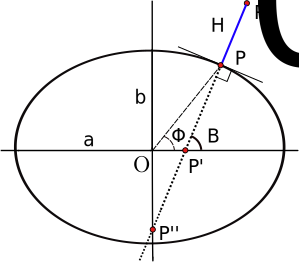
\includegraphics{fig/GeodeticHLat}
    \caption{Сечение эллипсоида --- эллипс. К определению геодезических широты $B$ и высоты $H$}
    \label{fig:GeodeticHLat}
\end{figure}
Геоодезическая широта $B$ (см. рисунок \ref{fig:GeodeticHLat}) для некоторой точки $P$ есть угол между опущенной из $P$ нормалью к эллипсоиду и плоскостью
экватора. Геодезическая долгота $L$ --- угол между плоскостью начального меридиана и плоскостью
меридиана точки $P$ (равна сферической долготе $\Lambda$). Геодезическая высота~$H$ --- (кратчайшее) 
расстояние от точки $P$ по нормали до поверхности эллипсоида (отрезок $PP_0$).

Важно отметить, что именно геодезическая система координат подразумевается, когда мы говорим
об определении физической поверхности Земли в единой системе координат. 
\begin{problem}
Подумайте, всегда ли в этой
системе координат поверхность Земли может быть определена однозначно? Какие недостатки у этой
системы координат?
\end{problem}

Геодезические координаты связаны с прямоугольными следующими соотношениями
\begin{align*}
    &X = \left( N + H \right)\cos{B}\cos{L},\\
    &Y = \left( N + H \right)\cos{B}\sin{L},\\
    &Z = \left( N + H - Ne^2 \right)\sin{B},
\end{align*}
где $N$ --- радиус кривизны первого вертикала, который, как известно из курса сфероидической
геодезии, вычисляется так
\begin{equation*}
    N = \frac{a}{\sqrt{1 - e^2\sin^2{B}}}.
\end{equation*}

На рисунке \ref{fig:GeodeticHLat} $N = P_0 P''$.

\begin{problem}
    Вспомните, что такое первый вертикал и что такое плоскость меридиана? Что такое главные радиусы
    кривизны эллипсоида?
\end{problem}

Геодезическая долгота $L$ совпадает со сферической
долготой $\Lambda$, если начала и ориентация координатных осей систем совпадают. 
Геоцентрическая широта отличается от геодезической (см. рисунок \ref{fig:GeodeticHLat}). На поверхности эллипсоида они связаны следующим
выражением
\begin{equation*}
    \tg{\Phi} = \left( 1 - e^2 \right)\tg{B}.
\end{equation*}

Геодезические широта и долгота отличаются от соответствующих астрономических координат, поскольку
направление отвесной линии отличается от направления нормали к эллипсоиду. Угол между направлением
отвесной линии и нормалью к эллипсоиду называется астрономо--геодезическим уклонением отвеса.
Удобно этот угол разложить на две составляющие --- проекции угла в плоскости первого вертикала
$\eta$  и в плоскости меридиана $\xi$, тогда
\begin{align*}
    &\xi = \phi - B,\\
    &\eta = \left( \lambda - L \right)\cos\phi.
\end{align*}
В дальнейшем мы познакомимся и с другими видами уклонения отвеса.

\section{Связь с другими науками}
\paragraph{Математика.}
Изучение гравитационного поля и фигуры Земли --- сложная задача. В ходе курса мы будет пользоваться
различными разделами математики, с некоторыми из которых вам придется познакомиться впервые:
\begin{itemize}
    \item векторный анализ,
    \item теория поля,
    \item теория ньютоновского потенциала,
    \item специальные функции,
    \item дифференциальные уравнения, обыкновенные и в частных производных,
    \item краевые задачи.
\end{itemize}
Исторически так сложилось, как и в случае теории математической обработки геодезических
измерений, обогатившей теорию вероятностей, теория фигуры Земли обогатила многие разделы математики,
которые теперь прочно служат её основой.

\paragraph{Геофизика и геология.} Гравитационное поле на поверхности Земли отражает распределение масс внутри
неё. И хотя, как мы очень скоро убедимся, одних только гравиметрических данных недостаточно для изучения 
внутреннего строения, они, наряду с другими геоифизическими методами, служат важным источником
информации.\par
Гравиметрический метод является одним из основных при поиске и разведке полезных ископаемых.
Высокоточные регулярные измерения используются для монторинга месторождений в процессе добычи нефти и газа.
\paragraph{Археология и строительство.} Локальная информация о гравитационном поле может быть
полезна для поиска пустот (карст), провалов, древних подземных ходов и тоннелей, объектов археологического
наследия.
\paragraph{Гляциология и уровень моря. Океанология.} Таяние ледников, вызванное изменением климата, уменьшает их
массу, следовательно, меняется и гравитационное поле. По спутниковым гравиметрическим данным (миссия GRACE) получены
важнейшие данные о ледниках Гренландии и Антарктиды. Таяние льдов вызывает рост среднего
уровня Мирового океана, следовательно, изменение высоты морской топографической поверхности, то есть
физической поверхности Земли. Эти процессы изучаются методом спутниковой альтиметрии.
\paragraph{Гидрология.} Перераспределение водных масс на всей поверхности Земли вызвано не только
таянием льдов, но и другими климатическими явлениями. Локальные измерения слы тяжести позволяют
изучать местный гидрологический режим, а спутниковые гравиметрические миссии --- региональный и даже
глобальный. 
\paragraph{Орбиты ИСЗ.} Для вычисления орбит искусственных спутников для определения его положения относительно центра
масс Земли необходимо знание гравитационного поля вне поверхности Земли (на высоте полета спутника). Этот нюанс свидетельствует
о том, что, казалось бы, чисто геометрический метод определения координат при помощи глобальных
навигационных спутниковых систем, на самом деле также связан с гравитационным полем.

Кроме всего вышеперечисленного, высокоточные измерения силы тяжести используются в метрологии и при
изучении геодинамических процессов, а также в других областях науки и техники.

\printbibliography
\end{document}
